\chapter{Organisation im Team}

Zu Beginn des Projekts haben wir unser Vorgehen auf Basis einer Literaturrecherche thematisch 
strukturiert und die anstehenden Aufgaben in Arbeitspakete unterteilt. Jedes Arbeitspaket wurde 
einem spezifischen Themenbereich zugeordnet, beispielsweise Datenanalyse- und aufbereitung, 
Labelling und Modelltraining.

Die Aufgaben innerhalb der Arbeitspakete wurden anschließend einzelnen Teammitgliedern 
zugewiesen, welche bis zum jeweils nächsten Termin bearbeitet wurden.

In unseren Internen Terminen hat zu zu Beginn jeder seinen aktuellen Stand seiner Arbeit vorgestellt. Im Anschluss wurden ggf. aufgetretene Probleme 
besprochen. Anschließend wurde anhand der aufgetretenen Probleme und des aktuellen Fortschritts 
die nächsten Aufgaben für das jeweilige Arbeitspaket erstellt und zugewiesen. So konnten wir 
flexibel auf die gegebenen Umstände reagieren. 

Die Zuständigkeiten für die jeweiligen Arbeitspakete können der folgenden Abbildung \ref{fig:Zeitentabelle}
entnommen werden. 

\begin{wrapfigure}{l}{1\linewidth}
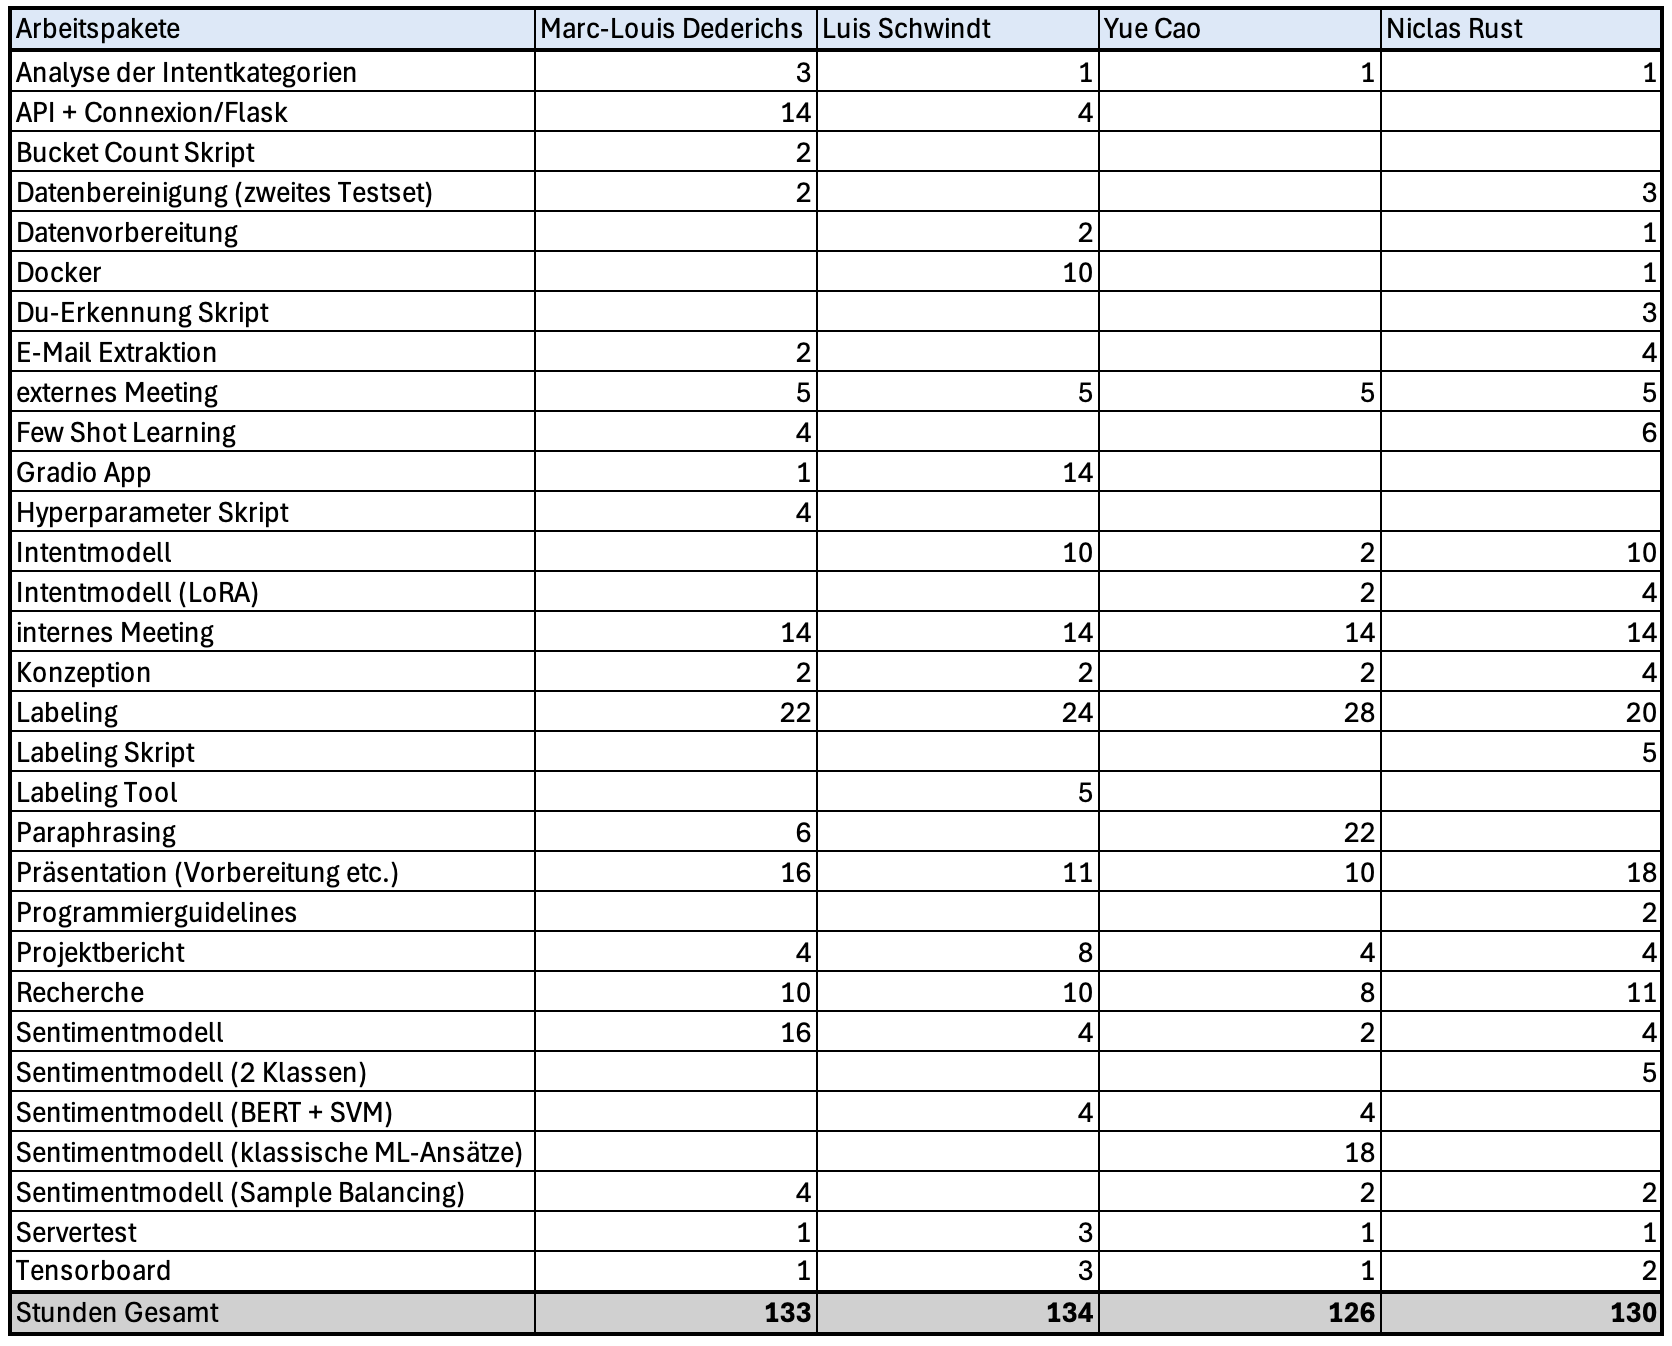
\includegraphics[width=\linewidth]{bilder/Zeitentabelle.png}
\caption[Zeitentabelle]{Zeitentabelle}
\label{fig:Zeitentabelle}
\end{wrapfigure}